\documentclass{article}
\usepackage{pgf-umlcd}
\usepackage{geometry}
\geometry{
  a2paper,
  total={680mm,1028mm},
  left=6cm,
  top=4cm,
}


\begin{document}
\section*{UML Class Diagram}
Alexander De Laurentiis (40050385)\\
Anoop Pukulakatt (40130695)\\
Vu Dang Khoa Trinh (40012738)

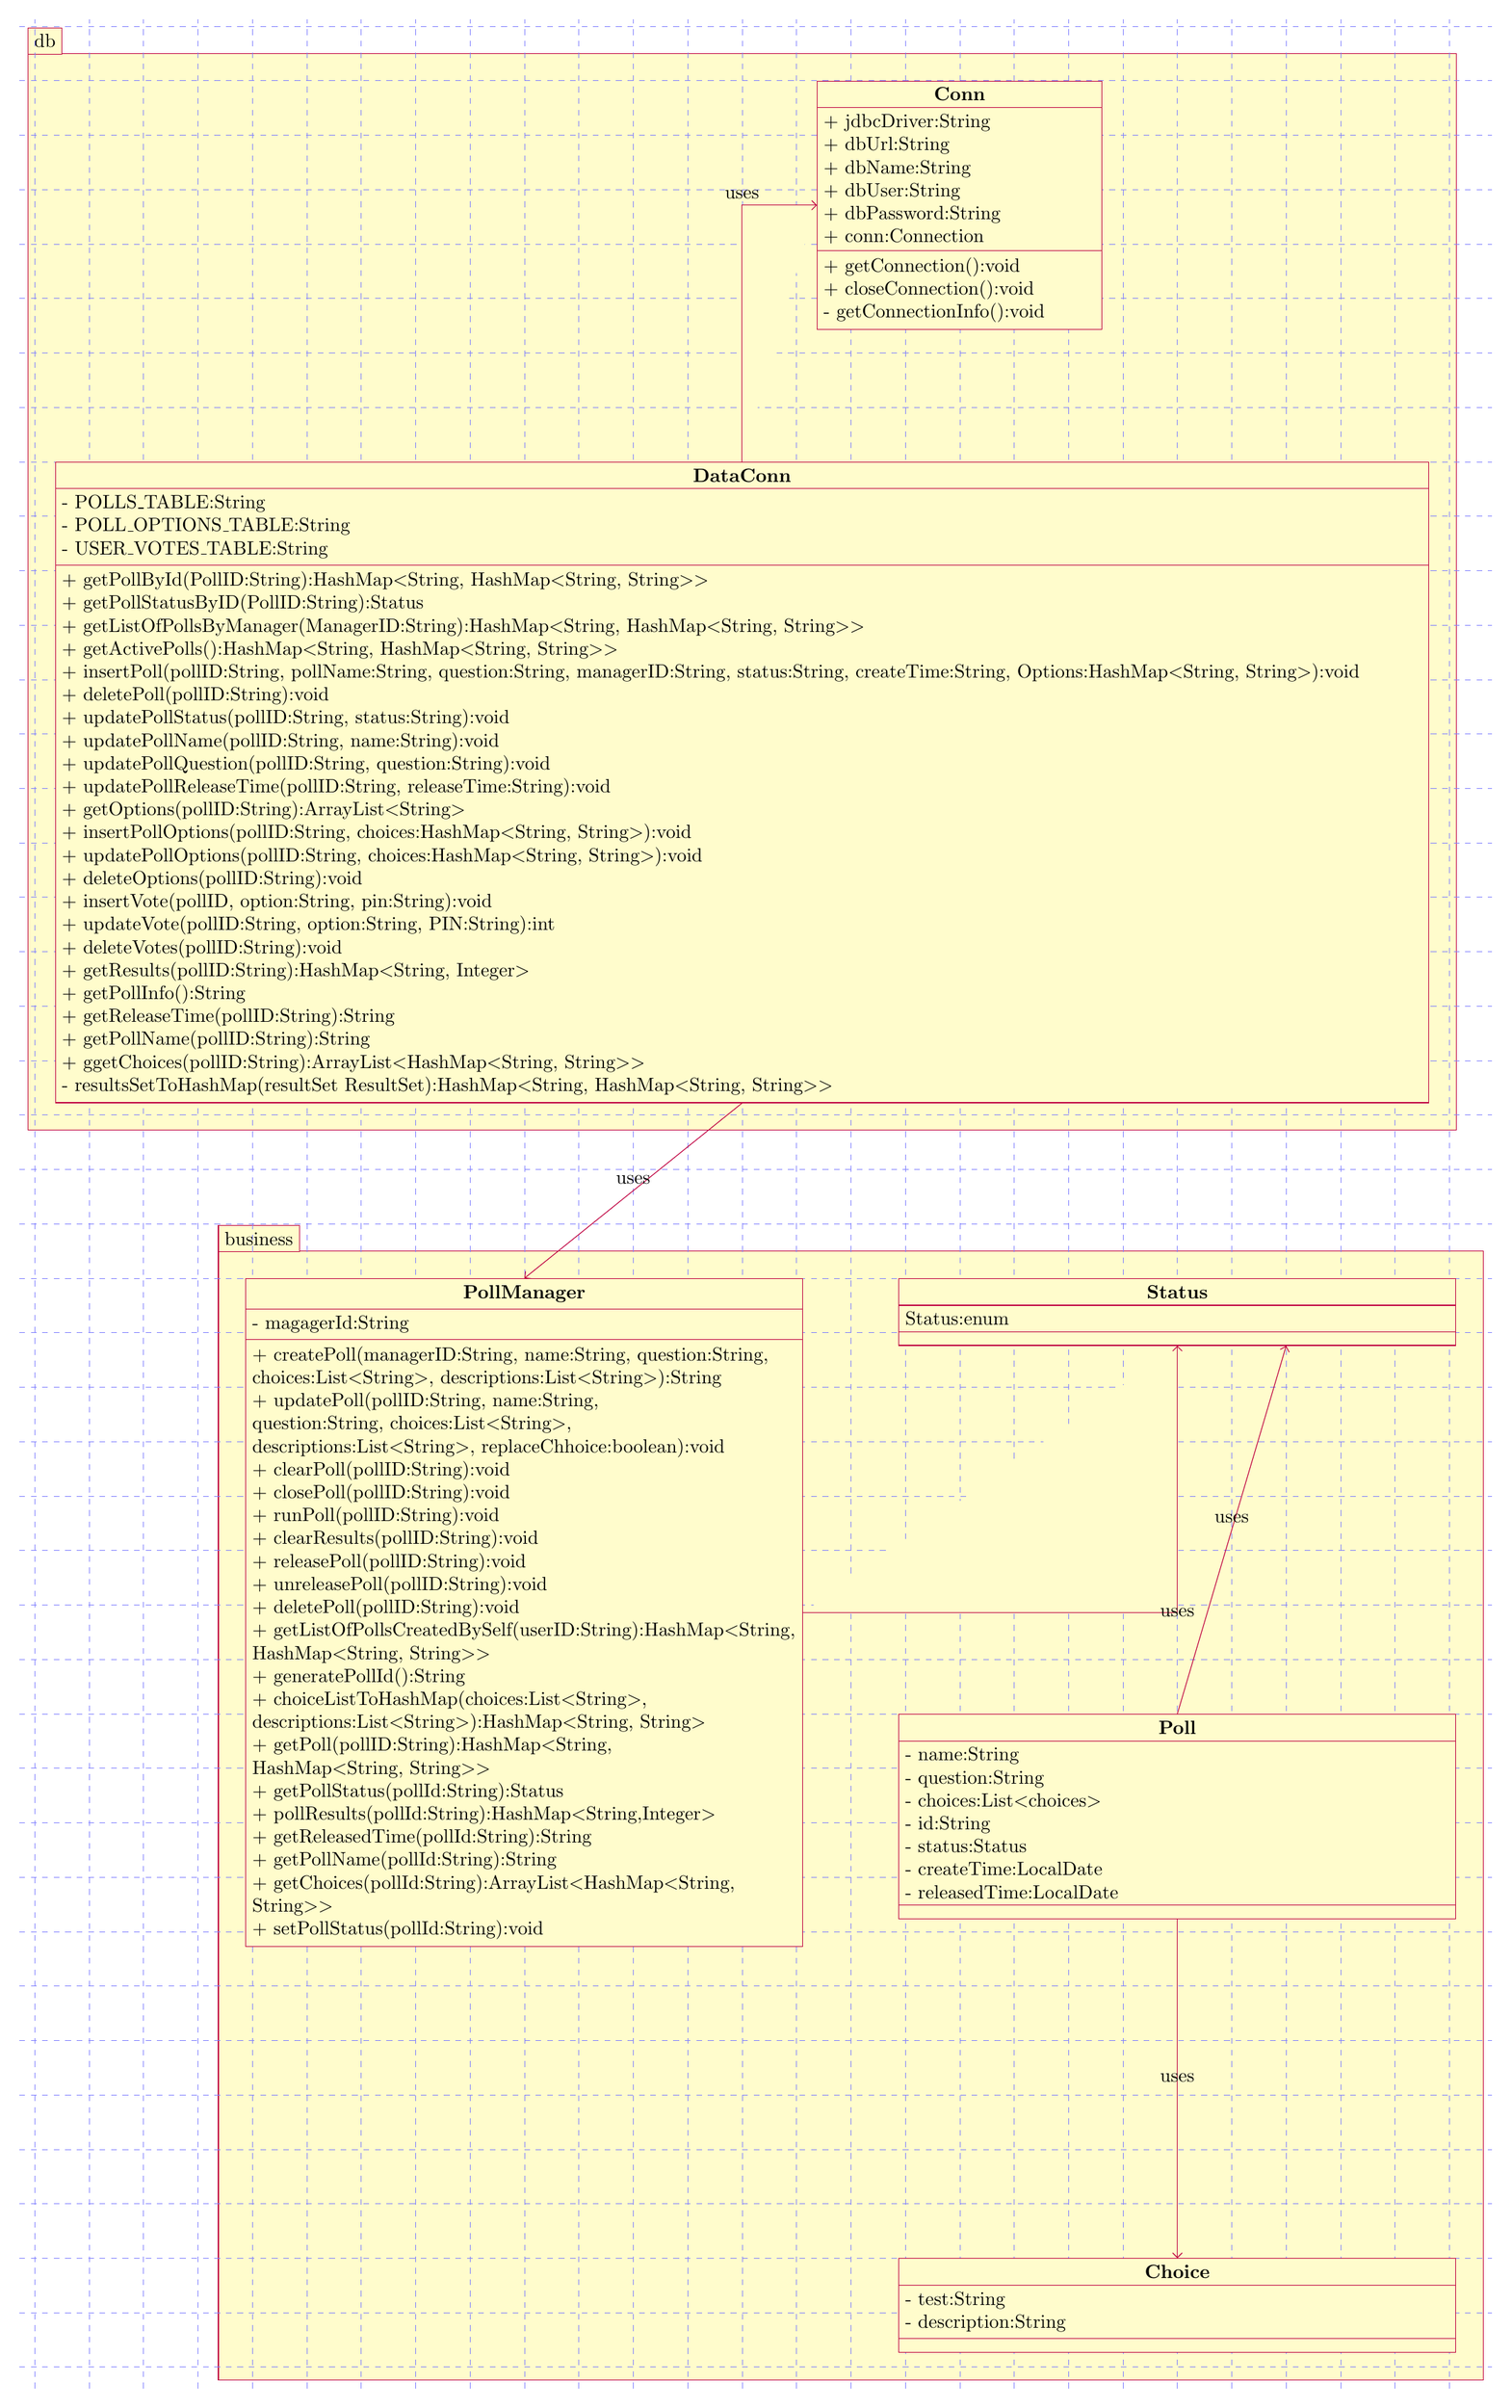
\begin{tikzpicture}[show background grid]
  % used classes
  % - Conn
  % - DataConn
  % - PollManager
  % - Status
  % - Poll
  % - Choice
  % No
  % - ballot
  % - vote
  % - voting user
  \begin{package}{db}
    \begin{class}[text width=5cm]{Conn}{0,0}
      \attribute{+ jdbcDriver:String}
      \attribute{+ dbUrl:String}
      \attribute{+ dbName:String}
      \attribute{+ dbUser:String}
      \attribute{+ dbPassword:String}
      \attribute{+ conn:Connection}
      \operation{+ getConnection():void}
      \operation{+ closeConnection():void}
      \operation{- getConnectionInfo():void}
    \end{class}
    \begin{class}[text width=25cm]{DataConn}{-4,-7}
      \attribute{- POLLS\_TABLE:String}
      \attribute{- POLL\_OPTIONS\_TABLE:String}
      \attribute{- USER\_VOTES\_TABLE:String}    
      \operation{+ getPollById(PollID:String):HashMap$<$String, HashMap$<$String, String$>>$}
      \operation{+ getPollStatusByID(PollID:String):Status}
      \operation{+ getListOfPollsByManager(ManagerID:String):HashMap$<$String, HashMap$<$String, String$>>$}
      \operation{+ getActivePolls():HashMap$<$String, HashMap$<$String, String$>>$}
      \operation{+ insertPoll(pollID:String, pollName:String, question:String, managerID:String, status:String, createTime:String, Options:HashMap$<$String, String$>$):void}
      \operation{+ deletePoll(pollID:String):void}
      \operation{+ updatePollStatus(pollID:String, status:String):void}
      \operation{+ updatePollName(pollID:String, name:String):void}
      \operation{+ updatePollQuestion(pollID:String, question:String):void}
      \operation{+ updatePollReleaseTime(pollID:String, releaseTime:String):void}
      \operation{+ getOptions(pollID:String):ArrayList$<$String$>$}
      \operation{+ insertPollOptions(pollID:String, choices:HashMap$<$String, String$>$):void}
      \operation{+ updatePollOptions(pollID:String, choices:HashMap$<$String, String$>$):void}
      \operation{+ deleteOptions(pollID:String):void}
      \operation{+ insertVote(pollID, option:String, pin:String):void}
      \operation{+ updateVote(pollID:String, option:String, PIN:String):int}
      \operation{+ deleteVotes(pollID:String):void}
      \operation{+ getResults(pollID:String):HashMap$<$String, Integer$>$}
      \operation{+ getPollInfo():String}
      \operation{+ getReleaseTime(pollID:String):String}
      \operation{+ getPollName(pollID:String):String}
      \operation{+ ggetChoices(pollID:String):ArrayList$<$HashMap$<$String, String$>>$}
      \operation{- resultsSetToHashMap(resultSet ResultSet):HashMap$<$String, HashMap$<$String, String$>>$}
    \end{class}
  \end{package}
  \begin{package}{business}
    \begin{class}[text width=10cm]{PollManager}{-8,-22}
      \attribute{- magagerId:String}
      \operation{+ createPoll(managerID:String, name:String, question:String, choices:List$<$String$>$, descriptions:List$<$String$>$):String}
      \operation{+ updatePoll(pollID:String, name:String, question:String, choices:List$<$String$>$, descriptions:List$<$String$>$, replaceChhoice:boolean):void}
      \operation{+ clearPoll(pollID:String):void}
      \operation{+ closePoll(pollID:String):void}
      \operation{+ runPoll(pollID:String):void}
      \operation{+ clearResults(pollID:String):void}
      \operation{+ releasePoll(pollID:String):void}
      \operation{+ unreleasePoll(pollID:String):void}
      \operation{+ deletePoll(pollID:String):void}
      \operation{+ getListOfPollsCreatedBySelf(userID:String):HashMap$<$String, HashMap$<$String, String$>$$>$}
      \operation{+ generatePollId():String}
      \operation{+ choiceListToHashMap(choices:List$<$String$>$, descriptions:List$<$String$>$):HashMap$<$String, String$>$}
      
      \operation{+ getPoll(pollID:String):HashMap$<$String, HashMap$<$String, String$>$$>$}
      \operation{+ getPollStatus(pollId:String):Status}
      \operation{+ pollResults(pollId:String):HashMap$<$String,Integer$>$}
      \operation{+ getReleasedTime(pollId:String):String}
      \operation{+ getPollName(pollId:String):String}
      \operation{+ getChoices(pollId:String):ArrayList$<$HashMap$<$String, String$>$$>$}
      \operation{+ setPollStatus(pollId:String):void}
    \end{class}
    \begin{class}[text width=10cm]{Status}{4,-22}
      \attribute{Status:enum}
      \operation{}
    \end{class}
    \begin{class}[text width=10cm]{Poll}{4,-30}
      \attribute{- name:String}
      \attribute{- question:String}
      \attribute{- choices:List$<$choices$>$}
      \attribute{- id:String}
      \attribute{- status:Status}
      \attribute{- createTime:LocalDate}    
      \attribute{- releasedTime:LocalDate}
    \end{class}
    \begin{class}[text width=10cm]{Choice}{4,-40}
      \attribute{- test:String}
      \attribute{- description:String}
    \end{class}
  \end{package}
  % Relations
  \draw [umlcd style,  <-] (Conn.west) -| node [ above,  black ]{ uses } (DataConn.north) ;
  \draw [umlcd style,  <-] (PollManager.north) -- node [ above,  black ]{ uses } (DataConn.south) ;
  \draw [umlcd style,  ->] (PollManager.east) -| node [ ,  black ]{ uses } (Status.south) ;
  \draw [umlcd style,  <-] (Status.south) ++(2,0) -- node [ above,  black ]{ uses } (Poll.north);
  \draw [umlcd style,  <-] (Choice.north) -- node [ above,  black ]{ uses } (Poll.south) ;
  
  
\end{tikzpicture}
\end{document}